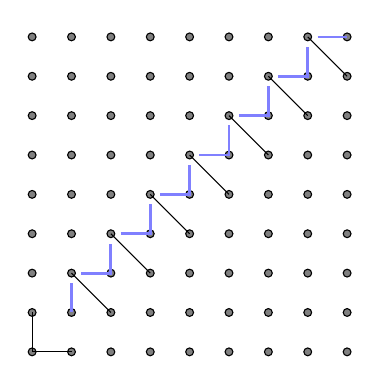
\begin{tikzpicture}
\tikzstyle{dot}=[draw,circle,fill=gray,scale=0.3];
\foreach \x in {0,...,8}
	\foreach \y in {0,...,8}
		\node[dot] at (\x*0.5,\y*0.5) {};

\draw (0,0) -- (0,0.5);
\draw (0,0) -- (0.5,0);
\draw (0.5,1) node (v1) {} -- (1,0.5);
\draw (1,1.5) node (v2) {} -- (1.5,1);
\draw (1.5,2) node (v3) {} -- (2,1.5);
\draw (2,2.5) node (v4) {} -- (2.5,2);
\draw (2.5,3) node (v5) {} -- (3,2.5);
\draw (3,3.5) node (v6) {} -- (3.5,3);
\draw (3.5,4) node (v8) {} -- (4,3.5);

\draw[draw=blue!50,line width=1pt] (0.5,0.5) -- (v1) -- (1,1) -- (v2) -- (1.5,1.5) -- (v3) -- (2,2) -- (v4) -- (2.5,2.5) -- (v5) -- (3,3) -- (v6) -- (3.5,3.5) node (v7) {}-- (v8) -- (4,4);
\end{tikzpicture}